\documentclass[Ligatures=TeX,table,brazil,svgnames,usetotalslideindicator,compress,10pt]{beamer}

\usetheme[titleformat=allsmallcaps]{metropolis}

\usepackage{polyglossia}
\setdefaultlanguage{brazil}
\disablehyphenation

\usepackage{minted}

\usetikzlibrary{arrows,positioning,calc}

\usepackage{graphicx}
\graphicspath{{./figuras/}}
\usepackage{subcaption}
\usepackage{xmpmulti}

%\usepackage{textpos}

%\usepackage{mdwlist}
%\usepackage{siunitx}
\usepackage{alltt}
%\usepackage{multicol}
\usepackage{xspace}
\usepackage{multirow}
\usepackage{amsmath}

\usepackage{cancel}

\newcommand{\setcoverbg}{
    \setbeamertemplate{background}
     {\includegraphics[width=\paperwidth,height=\paperheight]{backgrounds/coverbg}}
}
\newcommand{\setintersectionbg}{
    \setbeamertemplate{background}
     {\includegraphics[width=\paperwidth,height=\paperheight]{backgrounds/blank}}
}
\newcommand{\setsectionbg}{
    \setbeamertemplate{background}
     {\includegraphics[width=\paperwidth,height=\paperheight]{backgrounds/slidebg2}}
}

\setbeamertemplate{caption}{default}

\title{MCTA025-13 - Sistemas Distribuídos}
\subtitle{Arquiteturas de Sistemas Distribuídos}

\author{Emilio Francesquini}
\institute{Centro de Matemática, Computação e Cognição\\ Universidade Federal do ABC}
\date{18 de junho de 2018}

\begin{document}

\setcoverbg
\maketitle

\setsectionbg

\begin{frame}
  \frametitle{Disclaimer}
  \begin{itemize}
  \item Estes slides foram preparados para o curso de \textbf{Sistemas
      Distribuídos na UFABC}.
  \item Este material pode ser usado livremente desde que sejam
    mantidos, além deste aviso, os créditos aos autores e
    instituições.
  \item Estes slides foram adaptados daqueles originalmente preparados
    (e gentilmente cedidos) pelo professor \textbf{Daniel Cordeiro, da
      EACH-USP} que por sua vez foram baseados naqueles
    disponibilizados online pelos autores do livro ``Distributed
    Systems'', 3ª Edição em:
    \url{https://www.distributed-systems.net}.
  \end{itemize}
\end{frame}

\begin{frame}
  \frametitle{Arquiteturas}
  \begin{itemize}
  \item Estilos arquiteturais
  \item Arquiteturas de software
  \item Arquiteturas versus middleware
  \item Sistemas distribuídos autogerenciáveis
  \end{itemize}
\end{frame}

\begin{frame}
  \frametitle{Estilos arquiteturais}
  \begin{block}{Ideia básica}
    Um estilo é definido em termos de:
    \begin{itemize}
    \item componentes (substituíveis) com interfaces bem definidas
    \item o modo como os componentes são conectados entre si
    \item como os dados são trocados entre componentes
    \item como esses componentes e conectores são configurados conjuntamente em um sistema
    \end{itemize}
  \end{block}

  \begin{block}{Conector}
    Um mecanismo que intermedeia comunicação, coordenação ou cooperação entre componentes. Exemplo: recursos para chamadas de procedimento (remotos), mensagens ou \textit{streaming}.
  \end{block}
\end{frame}

\begin{frame}
  \frametitle{Estilos arquiteturais}
  \begin{block}{Ideia básica}
    Organize em componentes \alert{logicamente diferentes} e os distribua entre as máquinas disponíveis.
  \end{block}

  \includegraphics[scale=0.83]{02-01}

  (a)~Estilo em camadas é usado em sistemas cliente-servidor \newline
  (b)~Estilo orientado a objetos usado em sistemas de objetos distribuídos.

\end{frame}

\begin{frame}
  \frametitle{Estilos arquiteturais}
  \begin{block}{Observação}
    Desacoplar processos no \alert{espaço} (anônimos) e \alert{tempo} (assíncronos) pode levar a estilos diferentes.
  \end{block}

  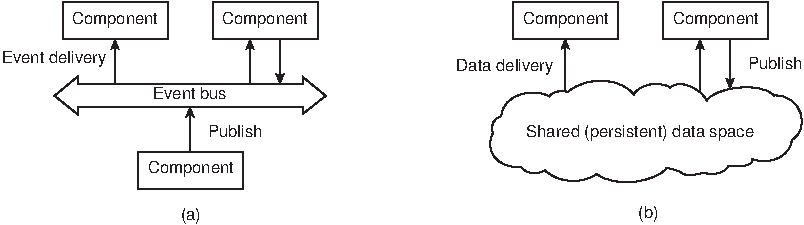
\includegraphics[scale=0.83]{02-02-antigo}

  (a)~Publish/subscribe [desaclopado no \alert{espaço}] \newline
  (b)~Espaço de dados compartilhados [desacoplado no \alert{espaço} e \alert{tempo}]

\end{frame}

\begin{frame}
  \frametitle{Arquiteturas centralizadas}
  \begin{block}{Características do modelo Cliente--Servidor}
    \begin{itemize}
    \item Existem processos que oferecem serviços (\alert{servidores})
    \item Existem processos que usam esses serviços (\alert{clientes})
    \item Clientes e servidores podem estar em máquinas diferentes
    \item Clientes seguem um modelo requisição/resposta ao usar os serviços
    \end{itemize}
  \end{block}

  \begin{center}
    \includegraphics{02-03}
  \end{center}

\end{frame}

\begin{frame}
  \frametitle{Arquiteturas multicamada}
  \begin{block}{Visão tradicional em três camadas}
    \begin{itemize}
    \item A \alert{camada de apresentação} contém o necessário para a aplicação poder interagir com o usuário
    \item A \alert{camada de negócio} contém as funções de uma aplicação
    \item A \alert{camada de dados} contém os dados que o cliente quer manipular através dos componentes da aplicação
    \end{itemize}
  \end{block}

  \pause

  \begin{alertblock}{Observação}
    Estas camadas são encontradas em muitos sistemas de informação distribuídos, que usam tecnologias de bancos de dados tradicionais e suas aplicações auxiliares.
  \end{alertblock}

\end{frame}

\begin{frame}
  \frametitle{Arquiteturas multicamada}
  \begin{center}
    \includegraphics{02-04}
  \end{center}
\end{frame}

\begin{frame}
  \frametitle{Exemplo: protocolos de comunicação}
  \begin{block}{Protocolo, serviço, interface}
    \includegraphics[width=\textwidth]{02-02}
  \end{block}
\end{frame}

\begin{frame}[fragile]
  \frametitle{Comunicação entre duas partes}
  \begin{exampleblock}{Servidor}
    \scriptsize
\begin{minted}{python}
from socket import *
s = socket(AF_INET, SOCK_STREAM)
(conn, addr) = s.accept()  # returns new socket and addr. client
while True:                # forever
  data = conn.recv(1024)   # receive data from client
  if not data: break       # stop if client stopped
  conn.send(str(data)+"*") # return sent data plus an "*"
conn.close()               # close the connection
\end{minted}
  \end{exampleblock}
  \begin{exampleblock}{Cliente}
        \scriptsize
\begin{minted}{python}
from socket import *
s = socket(AF_INET, SOCK_STREAM)
s.connect((HOST, PORT)) # connect to server (block until accepted)
s.send('Hello, world')  # send some data
data = s.recv(1024)     # receive the response
print data              # print the result
s.close()               # close the connection
\end{minted}
  \end{exampleblock}
\end{frame}

\begin{frame}
  \frametitle{Estilo orientado a objetos}
  \begin{block}{Essência}
    Componentes são objetos, conectados entre si usando chamadas de procedimentos. Objetos podem ser colocados em máquinas diferentes; chamadas, por tanto, devem executar usando a rede.
  \end{block}

  \begin{figure}
    \centering
    \includegraphics[width=.6\textwidth]{02-05a}
  \end{figure}

  \begin{block}{Encapsulamento}
    Dizemos que um objeto \emph{encapsula dados} e oferece \emph{métodos para os dados} sem revelar sua implementação.
  \end{block}
\end{frame}


\begin{frame}
  \frametitle{Estilo orientado a objetos}
  \begin{figure}
    \centering
    \includegraphics[width=.9\textwidth]{rmi}
  \end{figure}

  \begin{block}{Encapsulamento}
    Os objetos (e consequentemente dados e comportamentos) ficam
    distribuídos pelo sistema. Apesar do usuário fazer chamadas que
    são equivalentes a chamadas locais, elas podem estar sendo feitas
    em \alert{objetos remotos}.
  \end{block}
\end{frame}


\begin{frame}
  \frametitle{Arquiteturas RESTful} Vê um sistema distribuído como uma
  coleção de recursos que são gerenciados individualmente por
  componentes. Recursos podem ser adicionados, removidos, recuperados
  e modificados por aplicações (remotas).  \small
    \begin{enumerate}
    \item Recursos são identificados usando um único esquema de nomeação
    \item Todos os serviços oferecem a mesma interface
    \item Mensagens enviadas de ou para um serviço são auto-descritivas
    \item Após a execução de uma operação em um serviço, o componente esquece tudo sobre quem chamou a operação
    \end{enumerate}

  \begin{block}{Operações básicas}
    \begin{table}
      \centering
      \begin{tabular}{l|l}
        \alert{Operação} & \alert{Descrição} \\ \hline
        \texttt{PUT}                 & Cria um novo recurso \\
                         \texttt{GET} & Recupera o estado de um recurso usando um tipo de representação \\
                         \texttt{DELETE}& Apaga um recurso \\
                         \texttt{POST}& Modifica um recurso ao transferir um novo estado
      \end{tabular}
    \end{table}
  \end{block}
\end{frame}

\begin{frame}
  \frametitle{Exemplo: Amazon Simple Storage Service}
  \begin{block}{Essência}
    \alert{Objetos} (arquivos) são armazenados em \alert{buckets} (diretórios). Buckets não podem ser colocados dentro de outros buckets. Operações em \texttt{ObjectName} em \texttt{BucketName} requerem o seguinte identificador:
    \begin{center}
      \texttt{http://BucketName.s3.amazonaws.com/ObjectName}
    \end{center}
  \end{block}

  \begin{exampleblock}{Operações típicas}
    Todas as operações são realizadas com requisições HTTP:
    \begin{itemize}
    \item Criar um bucket/objeto: \texttt{PUT} + URI
    \item Listar objetos: \texttt{GET} em um nome de bucket
    \item Ler um objeto: \texttt{GET} em uma URI completa
    \end{itemize}
  \end{exampleblock}
\end{frame}

\begin{frame}
  \frametitle{Arquiteturas multicamada}
  \begin{description}
  \item[\alert{uma camada:}] configurações de terminal burro/mainframe
  \item[\alert{duas camadas:}] configuração cliente--servidor único.
  \item[\alert{três camadas:}] cada camada em uma máquina separada
  \end{description}

  \begin{alertblock}{Configurações tradicionais em duas camadas físicas:}
    \includegraphics[scale=0.83]{02-05}
  \end{alertblock}

\end{frame}


\begin{frame}
  \frametitle{Arquiteturas decentralizadas}

  \begin{description}
  \item[P2P estruturado] os nós são organizados seguindo uma estrutura de dados distribuída específica
  \item[P2P não-estruturado] os nós selecionam aleatoriamente seus vizinhos
  \item[P2P híbrido] alguns nós são designados, de forma organizada, a
    executar funções especiais
  \end{description}

  \pause
  \begin{alertblock}{Nota:}
    Praticamente todos os casos são exemplos de \alert{redes overlay}: dados são roteados usando conexões definidas pelos nós (\textit{Cf.} multicast em nível de aplicação)
  \end{alertblock}

\end{frame}

\begin{frame}
  \frametitle{Sistemas P2P Estruturados - Essência}

  \begin{itemize}
  \item A ideia é utilizar um índice \alert{não baseado na semântica dos
    dados}: cada conjunto de dados é associado unicamente a uma chave
    que, por sua vez, é usada como índice. A maneira mais comum de
    fazer isto é através de uma \alert{função de hash}.
    \begin{itemize}
    \item  \texttt{chave(dado) = hash(dado)}
    \end{itemize}
    O sistema P2P passa então a ser responsável apenas por associar
    chaves a valores ou , de maneira equivalente, lidar apenas com
    \textbf{pares (chave, valor)}.
  \end{itemize}

  \alert{Exemplo simples: Hipercubo:}

  A procura por um dado d com \alert{chave}
   $k \in \{0,1,2,...2^4-1\}$ causa o roteamento da busca para o nó
   com \alert{identificador} k.

  \vspace{-3em}
  \begin{figure}
  \centering
  \includegraphics[scale=0.2]{hypercube}
  \end{figure}
\end{frame}

\begin{frame}
  \frametitle{Sistemas P2P estruturados}

  \begin{block}{Ideia básica}
    Organizar os nós em uma \alert{rede overlay} estruturada, tal como um anel lógico, e fazer com que alguns nós se tornem responsáveis por alguns serviços baseado unicamente em seus IDs.
  \end{block}

  \begin{columns}

    \begin{column}{0.5\textwidth}
      \includegraphics[scale=0.83]{02-07}
    \end{column}

    \begin{column}{0.5\textwidth}

      \begin{block}{Nota}
        O sistema provê uma operação \alert{\verb~LOOKUP(key)~} que irá fazer o roteamento de uma requisição até o nó correspondente.
      \end{block}
    \end{column}
  \end{columns}
\end{frame}

\begin{frame}
  \frametitle{Chord}
  \begin{figure}
      \centering
      \includegraphics[scale=0.35]{chord}
    \end{figure}
\end{frame}

\begin{frame}
  \frametitle{Sistemas P2P estruturados}

  \begin{exampleblock}{Outro exemplo}
    Organize os nós em um espaço $d$-dimensional e faça todos os nós ficarem responsáveis por um dado em uma região específica. Quando um nó for adicionado, divida a região.
  \end{exampleblock}

  \begin{center}
    \includegraphics[scale=0.71]{02-08}
  \end{center}

\end{frame}


\begin{frame}
  \frametitle{Sistemas P2P não-estruturados}
  \begin{block}{Observação}
    Muitos sistemas P2P não-estruturados tentam manter um \alert{grafo aleatório}.
  \end{block}

  \begin{block}{Princípio básico}
    Cada nó deve contactar um outro nó selecionado aleatoriamente:

    \begin{itemize}
    \item Cada participante mantém uma \alert{visão parcial} da rede, consistindo de $c$ outros nós
    \item Cada nó $P$ seleciona periodicamente um nó $Q$ de sua visão parcial
    \item $P$ e $Q$ trocam informação \textbf{\&\&} trocam membros de suas respectivas visões parciais
    \end{itemize}
  \end{block}

  \vspace{-1em}
  \begin{alertblock}{Nota}
    Dependendo de como as trocas são feitas, não só a aleatoriedade
    mas também a \alert{robustez} da rede pode ser garantida.
  \end{alertblock}

\end{frame}

\begin{frame}
  \frametitle{O que é gossiping?}

  \begin{tabular}{@{}l@{}|l}
    {Thread ativa} & {Thread passiva} \\
    \begin{minipage}[b]{5.7cm}
      \begin{alltt}\fontsize{10}{10pt}\selectfont\bfseries
        \onslide<2->\alert{selectPeer}(\&B); \\
        \onslide<3->\alert{selectToSend}(\&bufs); \\
        \onslide<4->sendTo(B, bufs); \\
        \\
        \onslide<6->receiveFrom(B, \&bufr); \\
        \onslide<7->\alert{selectToKeep}(cache, bufr); \\
      \end{alltt}
    \end{minipage}
    &
    \begin{minipage}[b]{7cm}
      \begin{alltt}\fontsize{10}{10pt}\selectfont\bfseries
        \ \\
        \ \\
        \onslide<4->receiveFromAny(\&A, \&bufr); \\
        \onslide<5->\alert{selectToSend}(\&bufs); \\
        \onslide<6->sendTo(A, bufs); \\
        \onslide<7->\alert{selectToKeep}(cache, bufr); \\
      \end{alltt}
    \end{minipage}
  \end{tabular}

  \onslide<2->
  \small
  \begin{center}
    \framebox{%
      \begin{minipage}{11cm}
        \begin{description}[\alert{selectToSend}:]
        \item<2->[\alert{selectPeer}:] Seleciona aleatoriamente um vizinho de sua visão parcial.\hrule
        \item<3->[\alert{selectToSend}:] Seleciona \alert{$s$} entradas de seu cache local. \vspace*{0.2em}\hrule
        \item<7->[\alert{selectToKeep}:] (1)~Adiciona as entradas recebidas ao cache local. (2)~Remove os itens repetidos. (3)~Encolhe o tamanho do cache para \alert{$c$} (usando alguma estratégia).
        \end{description}
    \end{minipage}}
  \end{center}

\end{frame}

\begin{frame}
  \frametitle{Fundamento: amostragem  de peers usando gossip}

  \begin{alertblock}{}
    Unifica a visão parcial e o cache local $\Rightarrow$ troca os vizinhos
  \end{alertblock}

  \begin{tabular}{@{}l@{}|l}
    {Thread ativa} & {Thread passiva} \\
    \begin{minipage}[b]{5.7cm}
      \begin{alltt}\fontsize{9}{9pt}\selectfont\bfseries
        \onslide<2->\alert{selectPeer}(\&B); \\
        \onslide<3->\alert{selectToSend}(\&peers\_s); \\
        \onslide<4->sendTo(B, peers\_s); \\
        \\
        \onslide<6->receiveFrom(B, \&peers\_r); \\
        \onslide<7->\alert{selectToKeep}(pview, peers\_r); \\
      \end{alltt}
    \end{minipage}
    &
    \begin{minipage}[b]{7cm}
      \begin{alltt}\fontsize{9}{9pt}\selectfont\bfseries
        \ \\
        \ \\
        \onslide<4->receiveFromAny(\&A, \&peers\_r); \\
        \onslide<5->\alert{selectToSend}(\&peers\_s); \\
        \onslide<6->sendTo(A, peers\_s); \\
        \onslide<7->\alert{selectToKeep}(pview, peers\_r); \\
      \end{alltt}
    \end{minipage}
  \end{tabular}

  \onslide<2->
  \small
  \begin{center}
    \framebox{%
      \begin{minipage}{11cm}
        \begin{description}[\alert{selectToSend}:]
        \item<2->[\alert{selectPeer}:] Seleciona aleatoriamente um vizinho. \hrule
        \item<3->[\alert{selectToSend}:] Seleciona \alert{$s$} referências a vizinhos. \vspace*{0.2em}\hrule
        \item<7->[\alert{selectToKeep}:] (1)~Adiciona as referências recebidas à visão parcial. (2)~Remove as refs. repetidas.
          (3)~Encolhe o tamanho da visão para \alert{$c$}, removendo aleatoriamente as refs enviadas (mas nunca as recebidas).
        \end{description}
    \end{minipage}}
  \end{center}

\end{frame}

\begin{frame}
  \frametitle{Gerenciamento de topologia em redes de overlay}
  \begin{block}{Ideia básica}
    Distinguir duas camadas: (1)~mantém uma visão parcial aleatória na camada inferior; (2) seleciona quem manter nas visões parciais das camadas superiores.
  \end{block}

  \begin{figure}
    \centering
    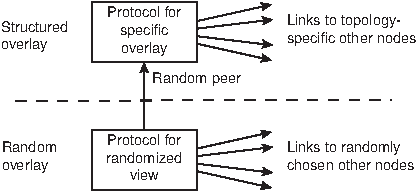
\includegraphics{02-10}
  \end{figure}

  \vspace{-0.5em}
  \begin{alertblock}{Nota}
    As camadas inferiores \alert{alimentam} as camadas superiores com nós escolhidos aleatoriamente; a camada superior é \alert{seletiva} para manter as referências.
  \end{alertblock}

\end{frame}

\begin{frame}
  \frametitle{Gerenciamento de topologia em redes de overlay}

  \begin{exampleblock}{Construindo um toro}
    Considere uma grade $N \times N$. Mantenha referências apenas aos \alert{vizinhos mais próximos}:
    \[\parallel (a_1,a_2) - (b_1,b_2) \parallel = d_1 + d_2\]
    \[d_i = \min\{N - |a_i - b_i|, |a_i - b_i|\}\]
  \end{exampleblock}

  \includegraphics[scale=0.65]{02-11}
\end{frame}

\mode<beamer>{%
  \begin{frame}
    \frametitle{Exemplo: criando clusters de nós}

    \alert{Ideia básica:} a todo nó $i$ é definido um
    \emph{identificador de grupo} $GID(i) \in \mathbb{N}$. O objetivo
    é particionar o overlay em \alert{componentes} disjuntos
    (clusters) tais que:

    \[dist(i,j) = \left\{\begin{array}{ll}
                           1 & \mbox{se $i$ e $j$ pertencem ao mesmo grupo [$GID(i) = GID(j)$]} \\
                           0 & \mbox{caso contrário} \\
                         \end{array}
                       \right.
                     \]
    \animate<0-22>
    \begin{center}
      \begin{tabular}{@{}c@{}c@{}c}
        \includegraphics[scale=0.2]{animacao-cap2/cluster-0.jpg} &
        \multiinclude[format=jpg,graphics={scale=0.2}]{animacao-cap2/cluster} &
        \includegraphics[scale=0.2]{animacao-cap2/cluster-19.jpg} \\
      \end{tabular}
    \end{center}

  \end{frame}}

\begin{frame}
  \frametitle{Superpeers}
  \begin{block}{Observação}
    Às vezes, selecionar alguns nós para realizar algum trabalho específico pode ser útil.
  \end{block}

  \begin{columns}\small
    \begin{column}{0.5\textwidth}
      \includegraphics{02-12}
    \end{column}

    \begin{column}{0.4\textwidth}

      \begin{exampleblock}{Exemplos:}
        \begin{itemize}
        \item Peers para manter um índice (para buscas)
        \item Peers para monitorar o estado da rede
        \item Peers capazes de configurar conexões
        \end{itemize}
      \end{exampleblock}

    \end{column}
  \end{columns}

\end{frame}

\begin{frame}
  \frametitle{Princípio de operação do Skype: A quer contactar B}
  \footnotesize
  \begin{block}{Tanto A quanto B estão na Internet pública}
    \begin{itemize}
    \item Uma conexão TCP é estabelecida entre A e B para envio de pacotes de controle
    \item A chamada real usa pacotes UDP entre as portas negociadas
    \end{itemize}
  \end{block}

  \pause
  \begin{block}{A está atrás de um firewall, B está na Internet pública}
    \begin{itemize}
    \item A configura uma conexão TCP (para os pacotes de controle) com um superpeer S
    \item S configura uma conexão TCP (para redirecionar os pacotes de controle) com B
    \item A chamada real usa pacotes UDP diretamente entre A e B
    \end{itemize}
  \end{block}

  \pause
  \begin{block}{Tanto A quanto B estão atrás de um firewall}
    \begin{itemize}
    \item A conecta com um superpeer S via TCP
    \item S configura uma conexão TCP com B
    \item Para a chamada real, outro superpeer é usado para funcionar como retransmissor (\alert{relay}): A (e B) configura a conexão com R
    \item A chamada é encaminhada usando duas conexões TCP, usando R como intermediário
    \end{itemize}
  \end{block}
\end{frame}

\begin{frame}
  \frametitle{Arquiteturas híbridas: cliente-servidor combinado com
    P2P}
  \begin{exampleblock}{Exemplo:}
    Arquiteturas de servidores de borda (\textit{edge-server}), utilizados com frequência como \alert{Content Delivery Networks} (redes de distribuição de conteúdo).
  \end{exampleblock}

  \begin{figure}
    \centering
    \includegraphics{02-13}
  \end{figure}
\end{frame}

\begin{frame}
  \frametitle{Arquiteturas híbridas: C--S com P2P -- BitTorrent}

  \begin{figure}
    \centering
    \includegraphics[scale=0.83]{02-14}
  \end{figure}

  \begin{block}{Ideia básica}
    Assim que um nó identifica de onde o arquivo será baixado, ele se junta a uma \alert{swarm} (multidão) de pessoas que, \alert{em paralelo}, receberão pedaços do arquivo da fonte e redistribuirão esses pedaços entre os outros.
  \end{block}
\end{frame}

\begin{frame}
  \frametitle{Arquiteturas versus Middleware}

  \begin{block}{Problema}
    Em muitos casos, arquiteturas/sistemas distribuídos são desenvolvidos de acordo com um estilo arquitetural específico. O estilo escolhido pode não ser o melhor em todos os casos $\Rightarrow$ é necessário \alert{adaptar o comportamento do middleware} (dinamicamente).
  \end{block}

  \begin{exampleblock}{Interceptors}
    Interceptam o fluxo de controle normal quando um \alert{objeto remoto} for invocado.
  \end{exampleblock}

\end{frame}


\begin{frame}
  \frametitle{Interceptors}
  \begin{figure}
    \centering
    \includegraphics[scale=0.83]{02-15}
  \end{figure}
\end{frame}

\begin{frame}
  \frametitle{Middleware adaptativo}
  \begin{itemize}
  \item \alert{Separação de interesses}: tente separar as
    \alert{funcionalidades extras} e depois \alert{costurá-las} em uma
    única implementação $\Rightarrow$ aplicabilidade restrita (\textit{toy examples})
  \item \alert{Reflexão computacional}: deixe o programa inspecionar-se em tempo de execução e adaptar/mudar suas configurações dinamicamente, se necessário  $\Rightarrow$ ocorre principalmente no nível da linguagem, aplicabilidade não é muito clara.
  \item \alert{Projeto baseado em componentes}: organize uma aplicação distribuída em componentes que podem ser substituídos dinamicamente quando necessário  $\Rightarrow$ causa muitas e complexas interdependências entre componentes.

  \end{itemize}
\end{frame}

\begin{frame}
  \frametitle{Sistemas distribuídos autogerenciáveis}
  \begin{block}{Observação}
    A distinção entre arquiteturas de sistemas e arquiteturas de
    software fica confusa quando \alert{adaptação automática} deve ser
    considerada:
  \end{block}

  \begin{itemize}
  \item Autoconfiguração
  \item Autogerenciamento
  \item Autocura
  \item Auto-otimização
  \item Auto-*
  \end{itemize}
\end{frame}

\begin{frame}
  \frametitle{Regulação por feedback}
  \textbf{Governador centrífugo}

 \begin{columns}

    \begin{column}{0.7\textwidth}
      \includegraphics[width=\textwidth]{steam}
    \end{column}

    \begin{column}{0.4\textwidth}
      \begin{itemize}
      \pause
      \item
      Criado em \textbf{1788} por \alert{James Watt}.
      \pause
      \item
      Controla a admissão de vapor no cilindro de máquinas a vapor.
      \end{itemize}
    \end{column}
  \end{columns}

\end{frame}


\begin{frame}
  \frametitle{Modelo de regulação por feedback}
  \begin{block}{}
    Em muitos casos, sistemas auto-* são organizados como um
    \alert{sistema de regulação por feedback}
  \end{block}

  \begin{figure}
    \centering
    \includegraphics{02-16}
  \end{figure}
\end{frame}



\end{document}
